\chapter{L'Algoritmo}
\paragraph{Attenzione:} per brevità, verr\'a trattato estensivamente nella descrizione solo il caso in cui B sia pi\'u alto di A, il caso inverso, comunque implementato nel codice, \'e simmetrico al presente e verrà presentato all'interno di parentesi quadre, in forma breve, per completezza.
Il Tempo indicato come sotto titolo ad ogni sezione è il risultato dell'analisi teorica del codice.


\section{Fase Preliminare ( SOLO VERSIONE DEMO )}
$\mathbf{Tempo: O(n)}$\\ 	\\
Nella fase preliminare l'algoritmo crea o da un Array attraverso il metodo \emph{createAVLTreeByArray()} o in maniera pseudo random 2 alberi AVL attraverso la funzione \emph{generateRandomAVLTree} ( contenuta in ProjUtilities).
Il presente metodo, per quanto veloce possa essere \'e l'unico il cui tempo di esecuzione sia pari ad un O(n). Chiaramente \'e un metodo esistente solo nella DEMO dell'algoritmo mentre la sua implementazione pura non prevede affatto questa parte ragion per cui nel calcolo totale ho ignorato tale risultato.
\newline
\newline

% Albero A
\paragraph{Albero A:}
\begin{center}
	\begin{tikzpicture}[level/.style={sibling distance=80mm/#1}]
	\node [circle,draw] {5}
	child {
		node [circle,draw] {2}
		child {node [circle,draw] {1}
		}
		child {
			node [circle,draw]{3}
		}
	}
	child {node [circle,draw] {6}
		child {node [circle,draw]  {4}
		}
		child {node [circle,draw]  {7}
			child {node [circle, draw]  {7}} 
			child {node [circle, draw]  {8}}
		}
	};
	
	\end{tikzpicture}
\end{center}

% Albero B
\paragraph{\newline Albero B: \newline}

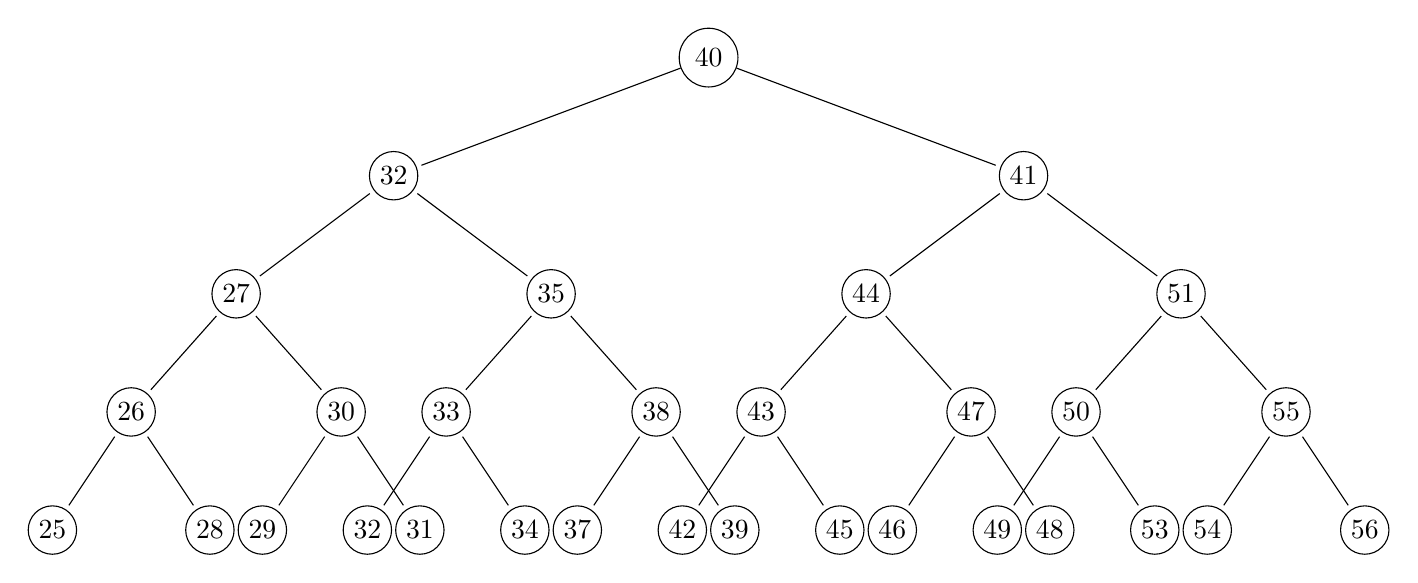
\begin{tikzpicture}[level/.style={sibling distance=80mm/#1, inner sep=2, outer sep=2}]
\node [circle,draw] {40}
child {
	node [circle,draw] {32} % sotto-albero sinistro
	child {
		node [circle,draw]{27}
		child {node [circle,draw] {26}
			child {node [circle,draw] {25}
			}
			child{node [circle,draw] {28}
			}	
		}
		child{node [circle,draw] {30}
			child {node [circle,draw] {29}
			}
			child{node [circle,draw] {31}
			}	
		}	
	}
	child {
		node [circle,draw]{35}
		child {node [circle,draw] {33}
			child {node [circle,draw] {32}
			}
			child{node [circle,draw] {34}
			}	
		}
		child{node [circle,draw] {38}
			child {node [circle,draw] {37}
			}
			child{node [circle,draw] {39}
			}	
		}	
	}
}
child {node [circle,draw] {41} % sotto-albero destro
	child {
		node [circle,draw]{44}
		child {node [circle,draw] {43}
			child {node [circle,draw] {42}
			}
			child{node [circle,draw] {45}
			}	
		}
		child{node [circle,draw] {47}
			child {node [circle,draw] {46}
			}
			child{node [circle,draw] {48}
			}	
		}	
	}
	child {
		node [circle,draw]{51}
		child {node [circle,draw] {50}
			child {node [circle,draw] {49}
			}
			child{node [circle,draw] {53}
			}	
		}
		child{node [circle,draw] {55}
			child {node [circle,draw] {54}
			}
			child{node [circle,draw] {56}
			}	
		}	
	}
};

\end{tikzpicture}

\newpage


\section{Confronto}
$\mathbf{Tempo: O(c)}$\\ 	\\
L'algoritmo, attraverso il metodo "getTreeHeight()" ottiene l'altezza dei due alberi AVL e ne salva il contenuto in due variabili $H_a$ ed $H_b$. ( Tale richiesta ovviamente impiega un Tempo costante quindi assimilabile ad un O(1)). Con queste variabili salvate effettua un piccolo e breve confronto per stabilire quali dei due alberi sia il pi\'u alto il risultato di tale confronto è alla base di tutto l'algoritmo. 
Per ipotesi, dal confronto risulta che A possegga un'altezza pari a 3 mentre l'albero B di 4.

\section{Ricerca del massimo di A}
$\mathbf{Tempo: O(log(n))}$\\ 	\\
L'idea alla base dell'algoritmo \'e quella di cercare di eseguire meno operazioni possibili, quindi, rispetto ad una prima idea naive che consisteva semplicemente nell'inserire i singoli nodi da un albero all'altro, si cerca invece di innestare per intero l'albero pi\'u basso, per ipotesi A, in quello pi\'u alto.
Per far ci\'o \'e necessario trovare un nodo che ci consenta di fare tale operazione senza sbilanciare troppo l'albero altrimenti il vantaggio dell'innesto dell'albero andrebbe perso nelle tante operazioni di rotazioni e di inserimento. L'attuale \emph{aim} quindi sarebbe cercare un nodo al quale si possa innestare l'intero albero A. Quel nodo fa effettivamente già parte di A in quanto se scegliessimo il Massimo di A l'intero albero potrebbe esservi innestato come figlio sinistro. Ora per\'o va cercato nell'albero B un nodo R dove innestare il nuovo albero così creato.
Dall'esempio sopra riportato il massimo di A, conservato nel suo nodo pi\'u a destra, \'e pari ad 8.
\newline[Se A fosse più alto di B allora si dovrebbe cercare invece il minimo di B, infatti si può innestare l'intero albero B alla destra del suo stesso minimo. Quindi il Nodo R non apparterrà a B in questa ipotesi bensì ad A]

\section{Ricerca del Nodo R}
$\mathbf{Tempo: O(log(n))}$\\ 	\\
Il prossimo \emph{aim} consiste nel trovare il nodo R di B dove innestare l'albero A cos\'i ri-arrangiato e fare tutto ci\'o senza sbilanciare troppo l'albero B. Una soluzione \'e riutilizzare l'informazione sull'altezza dell'albero A poich\'e sicuramente se riuscissimo ad innestare l'albero ad un nodo di altezza eguali o, nella peggiore delle ipotesi, maggiore di una singola unità,  ci\'o ci consentirebbe di  ottenere un albero B non troppo sbilanciato. Nell'ipotesi di B più alto di A ovviamente i candidati sarebbero 2 un nodo appartenente alla parte sinistra dell'albero ed uno alla destra. Poich\'e il nostro obbiettivo \'e innestare un albero con chiavi tutte minori di B sicuramente il candidato ideale \'e proprio il nodo della parte sinistra dell'albero. Tale nodo sarà per noi il nodo R. Nell'esempio il nodo che corrisponde a detti criteri \'e propri il figlio sinistro della radice (32).
\newline[Nell'ipotesi A più alto di B il candidato si trova nella parte destra dell'albero di A. Sfruttando il fatto che B ha tutte chiavi maggiori di A è ottimale trovare un nodo nella parte destra di A che di fatti sarà sicuramente maggiore di A e minore di B]
\section{Eliminazione del sotto-albero del nodo R}
$\mathbf{Tempo: O(c)}$\\ 	\\
Nella peggiore delle ipotesi il nodo R ha un figlio sulla sua destra e sulla sua sinistra quindi sarebbe necessario trovare un modo con cui innestare l'intero albero come figlio del nodo R senza però violare la proprietà degli Alberi Binari di Ricerca per cui ogni nodo non pu\'o avere pi\'o di due figli. Una buona strategia quindi consisterebbe nell'eliminazione del sotto albero di R ( con R incluso ) ( operazione che impiega $O(log(n))$ ) sostituire quindi a quel nodo il Massimo di A, con l'intero albero di A come suo figlio sinistro.
Dall'esempio segue l'albero B senza il nodo R ed il sotto-albero di R:
[Scegliendo come nodo R il candidato alla destra di A il nuovo albero da innestare in A avrà come radice il minimo di B, alla sua destra l'intero albero B e alla sua sinistra appunto il nodo R con suo relativo sotto-albero]
\newpage

%Albero B - Nodo R e suo relativo sotto-albero
\paragraph{Albero B privato del Nodo R con relativo sotto-albero: \newline \newline}
\begin{center}
	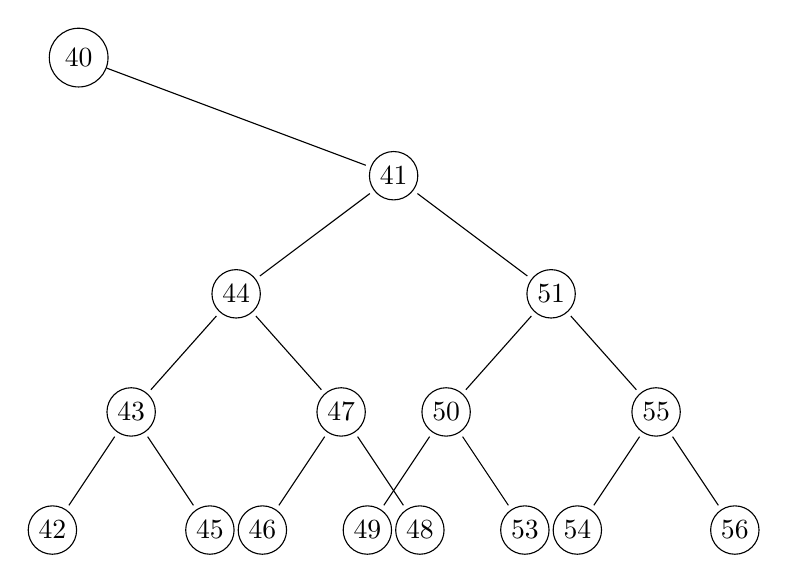
\begin{tikzpicture}[level/.style={sibling distance=80mm/#1, inner sep=2, outer sep=2}]
	\node [circle,draw] {40}
	child [missing]
	child {node [circle,draw] {41} % sotto-albero destro
		child {
			node [circle,draw]{44}
			child {node [circle,draw] {43}
				child {node [circle,draw] {42}
				}
				child{node [circle,draw] {45}
				}	
			}
			child{node [circle,draw] {47}
				child {node [circle,draw] {46}
				}
				child{node [circle,draw] {48}
				}	
			}	
		}
		child {
			node [circle,draw]{51}
			child {node [circle,draw] {50}
				child {node [circle,draw] {49}
				}
				child{node [circle,draw] {53}
				}	
			}
			child{node [circle,draw] {55}
				child {node [circle,draw] {54}
				}
				child{node [circle,draw] {56}
				}	
			}	
		}
	};
	
	\end{tikzpicture}
\end{center}

%Nodo R e suo relativo sotto-albero
\paragraph{ \newline \newline Nodo R e suo Sotto-albero: \newline \newline}
\begin{center}
	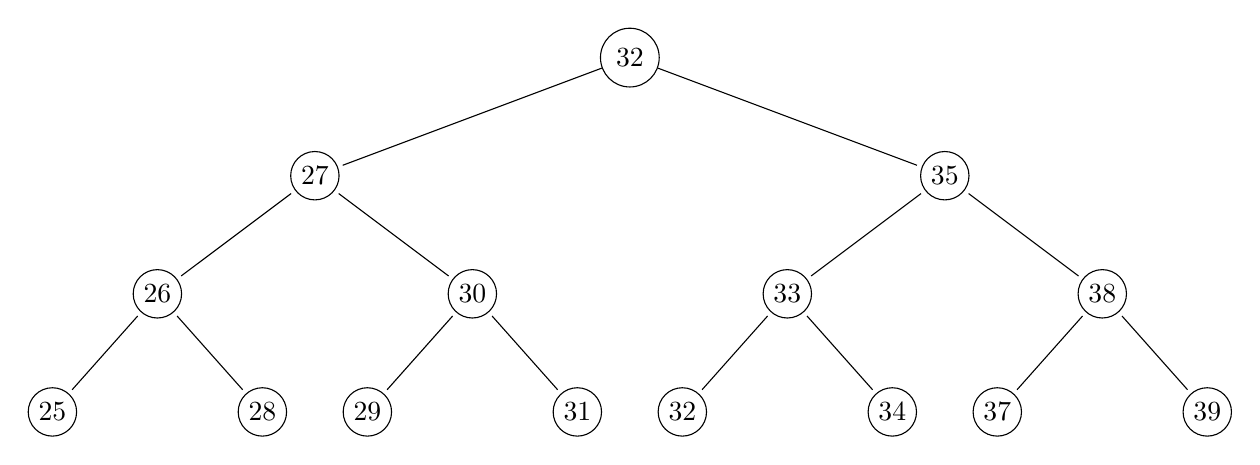
\begin{tikzpicture}[level/.style={sibling distance=80mm/#1, inner sep=2, outer sep=2}]
	\node [circle,draw] {32} % sotto-albero sinistro
	child {
		node [circle,draw]{27}
		child {node [circle,draw] {26}
			child {node [circle,draw] {25}
			}
			child{node [circle,draw] {28}
			}	
		}
		child{node [circle,draw] {30}
			child {node [circle,draw] {29}
			}
			child{node [circle,draw] {31}
			}	
		}	
	}
	child {
		node [circle,draw]{35}
		child {node [circle,draw] {33}
			child {node [circle,draw] {32}
			}
			child{node [circle,draw] {34}
			}	
		}
		child{node [circle,draw] {38}
			child {node [circle,draw] {37}
			}
			child{node [circle,draw] {39}
			}	
		}	
	};
	\end{tikzpicture}
\end{center}

%TempA senza nodo R e suo relativo sotto-albero
\paragraph{ \newline \newline Albero A Riarrangiato: \newline \newline}
\begin{center}
	\begin{tikzpicture}[level/.style={sibling distance=80mm/#1}]
	\node [circle,draw] {8}
	child{node [circle,draw] {5}
		child {
			node [circle,draw] {2}
			child {node [circle,draw] {1}
			}
			child {
				node [circle,draw]{3}
			}
		}
		child {node [circle,draw] {6}
			child {node [circle,draw]  {4}
			}
			child {node [circle,draw]  {7}
				child {node [circle, draw]  {7}} 
				child [missing]
			}
		}
	}
	child [missing]{};
	
	\end{tikzpicture}
\end{center}


%TempA
\paragraph{ Nuovo Albero da Innestare in B: \newline}
\begin{center}
	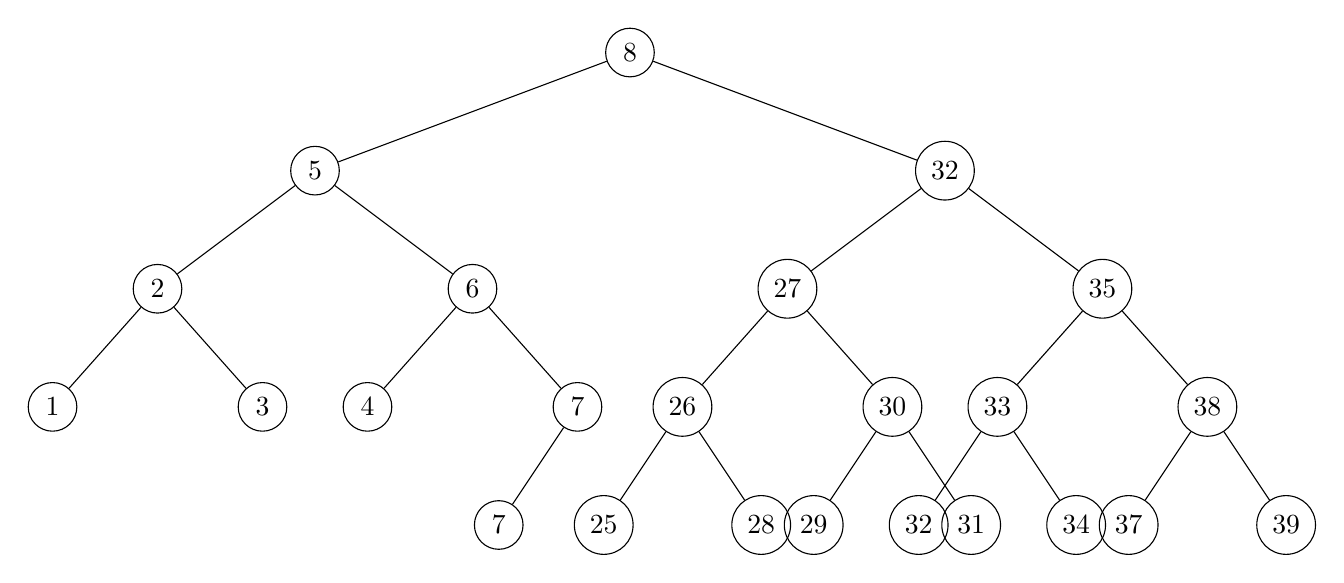
\begin{tikzpicture}[level/.style={sibling distance=80mm/#1}]
	\node [circle,draw] {8}
	child{node [circle,draw] {5}
		child {
			node [circle,draw] {2}
			child {node [circle,draw] {1}
			}
			child {
				node [circle,draw]{3}
			}
		}
		child {node [circle,draw] {6}
			child {node [circle,draw]  {4}
			}
			child {node [circle,draw]  {7}
				child {node [circle, draw]  {7}} 
				child [missing]
			}
		}
	}
	child {
		node [circle,draw] {32} % Nodo R con suo Sotto-Albero
		child {
			node [circle,draw]{27}
			child {node [circle,draw] {26}
				child {node [circle,draw] {25}
				}
				child{node [circle,draw] {28}
				}	
			}
			child{node [circle,draw] {30}
				child {node [circle,draw] {29}
				}
				child{node [circle,draw] {31}
				}	
			}	
		}
		child {
			node [circle,draw]{35}
			child {node [circle,draw] {33}
				child {node [circle,draw] {32}
				}
				child{node [circle,draw] {34}
				}	
			}
			child{node [circle,draw] {38}
				child {node [circle,draw] {37}
				}
				child{node [circle,draw] {39}
				}	
			}	
		}
	};
	
	\end{tikzpicture}
\end{center}



\section{Innesto del Sotto-albero R}
$\mathbf{Tempo: O(c)}$\\ 
Ora il il nuovo nodo così innestato rimane sprovvisto di figlio destro. Sfruttando la propriet\'a che ogni chiave dell'albero B \'e maggiore delle chiavi dell'albero di A possiamo innestare come figlio destro il nodo R con il suo intero sotto albero. 
[L'albero così creato in precedenza può essere inserito come figlio destro del padre di R senza perciò violare alcuna proprietà degli Alberi AVL salvo l'altezza che verrà subito aggiornata]

%Alberi Concatenati:
\paragraph{Alberi Concatenati:}
\begin{center}
	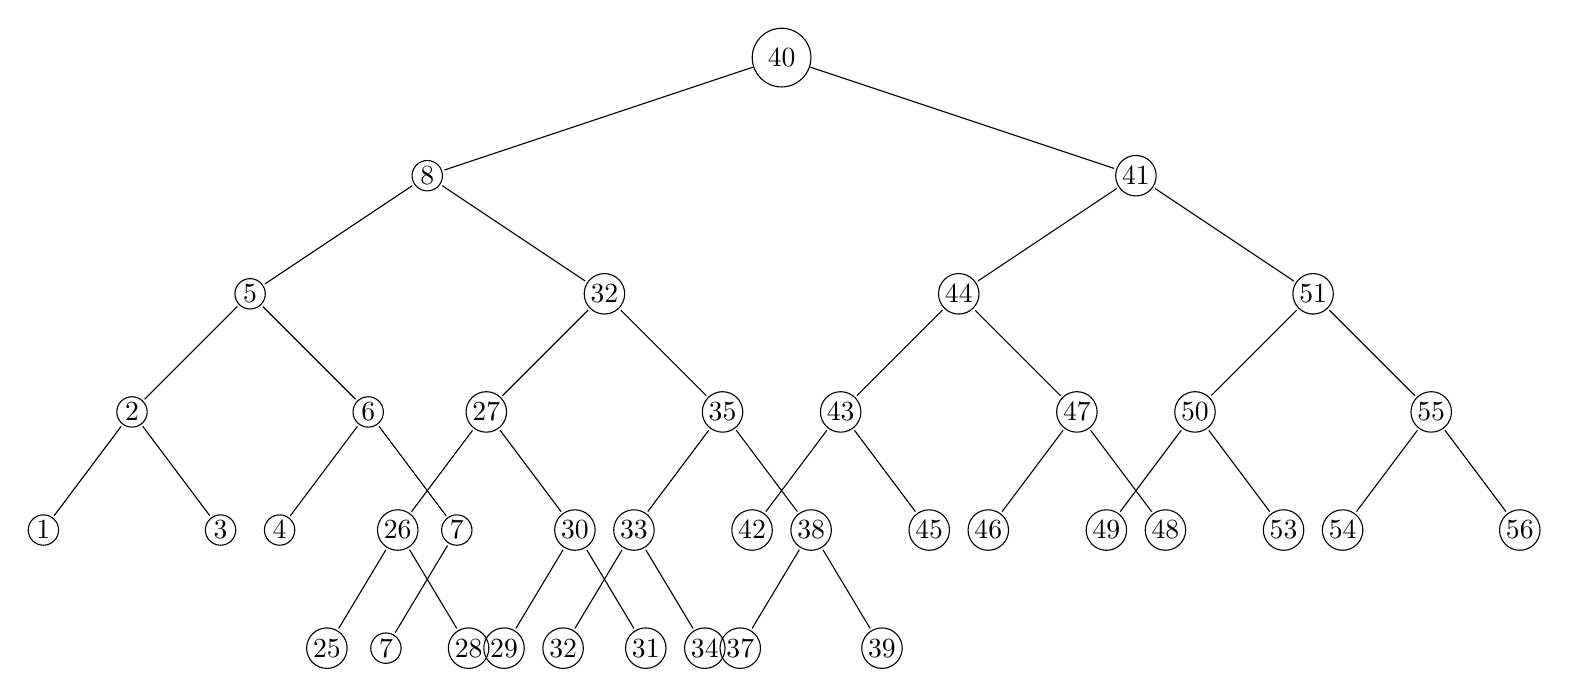
\begin{tikzpicture}[level/.style={sibling distance=90mm/#1, inner sep=1, outer sep=1}]
	\node [circle,draw] {40}
	child {
		node [circle,draw] {8}
		child{node [circle,draw] {5}
			child {
				node [circle,draw] {2}
				child {node [circle,draw] {1}
				}
				child {
					node [circle,draw]{3}
				}
			}
			child {node [circle,draw] {6}
				child {node [circle,draw]  {4}
				}
				child {node [circle,draw]  {7}
					child {node [circle, draw]  {7}} 
					child [missing]
				}
			}
		}
		child {
			node [circle,draw] {32} % Nodo R con suo Sotto-Albero
			child {
				node [circle,draw]{27}
				child {node [circle,draw] {26}
					child {node [circle,draw] {25}
					}
					child{node [circle,draw] {28}
					}	
				}
				child{node [circle,draw] {30}
					child {node [circle,draw] {29}
					}
					child{node [circle,draw] {31}
					}	
				}	
			}
			child {
				node [circle,draw]{35}
				child {node [circle,draw] {33}
					child {node [circle,draw] {32}
					}
					child{node [circle,draw] {34}
					}	
				}
				child{node [circle,draw] {38}
					child {node [circle,draw] {37}
					}
					child{node [circle,draw] {39}
					}	
				}	
			}
		}
	}
	child {node [circle,draw] {41} % sotto-albero destro
		child {
			node [circle,draw]{44}
			child {node [circle,draw] {43}
				child {node [circle,draw] {42}
				}
				child{node [circle,draw] {45}
				}	
			}
			child{node [circle,draw] {47}
				child {node [circle,draw] {46}
				}
				child{node [circle,draw] {48}
				}	
			}	
		}
		child {
			node [circle,draw]{51}
			child {node [circle,draw] {50}
				child {node [circle,draw] {49}
				}
				child{node [circle,draw] {53}
				}	
			}
			child{node [circle,draw] {55}
				child {node [circle,draw] {54}
				}
				child{node [circle,draw] {56}
				}	
			}	
		}
	};
	\end{tikzpicture}
\end{center}



\section{Aggiornamento dell'altezza}
$\mathbf{Tempo: O(log(n))}$\\ 	\\
Per costruzione il nodo così creato ( figlio sx albero A e figlio dx nodo R con relativo sotto-albero ) ha altezza eguali al vecchio nodo R, nella peggiore delle ipotesi differenti per una unità, si pu\'o chiedere quindi attraverso il metodo \emph{balInsert()} di ri-bilanciare l'albero così correggendo eventuali altezze discordi e così con l'ultima operazione in tempo $O(log(n))$ si ottengono i due alberi concatenati. Nell'esempio, il nuovo sotto-albero con radice in 8 \'e alto una singola unità in più del relativo sotto-albero radicato in 41 siccome è concesso uno sbilanciamento di una singola unità l'albero risulta difatti anche bilanciato di suo, completando il ciclo di operazioni in tempi logaritmici
